% Methodology section including data collection and data analysis technique
%no results or discussion here
%where the decisions made goes
%then discuss the decisions made in the discussion of framework

\chapter{Methodology}
To determine Trondheim's resilience requires an understanding of its technological, natural and social systems. Literature reviews including municipality policy and planning permission were carried out to determine the technological systems resilience. Natural systems resilience determination relied on research site observations and analysis of several  data-sets including: \cite{geonorge_stormflo_nodate} , \cite{kartverket_se_2021}, \cite{stormflo_database_stormflo_2021} and \cite{ipcc_sea_2021}. 
\paragraph{}
To determine Trondheim's social system resilience data collection utilising an online survey was carried out. The purpose of this survey included gathering data about local knowledge about sea level extremes, particularly the awareness level of the changing sea level extremes in Trondheim. To improve the design of this survey a pilot survey and focus group were first carried out.  

\section{Pilot Survey and Focus Group}

The pilot survey was conducted using 14 subjects on the 21st and the 25th of March, 2022. The subjects were classed as highly aware as they all had familiarity with changing sea level extremes in Brattøra. This was firstly due to being either Natural Resources Masters students or members of Trondheim Kayak Club and secondly as they had the project presented by the researcher in advance of responding to the survey. They were asked seven questions and three of them were used to attempt to determine the subjects' awareness of sea level extremes in Brattøra. The three figures below display the maps used when asking about the projected heights of sea level extremes.

\begin{figure} [h!]
    \centering
    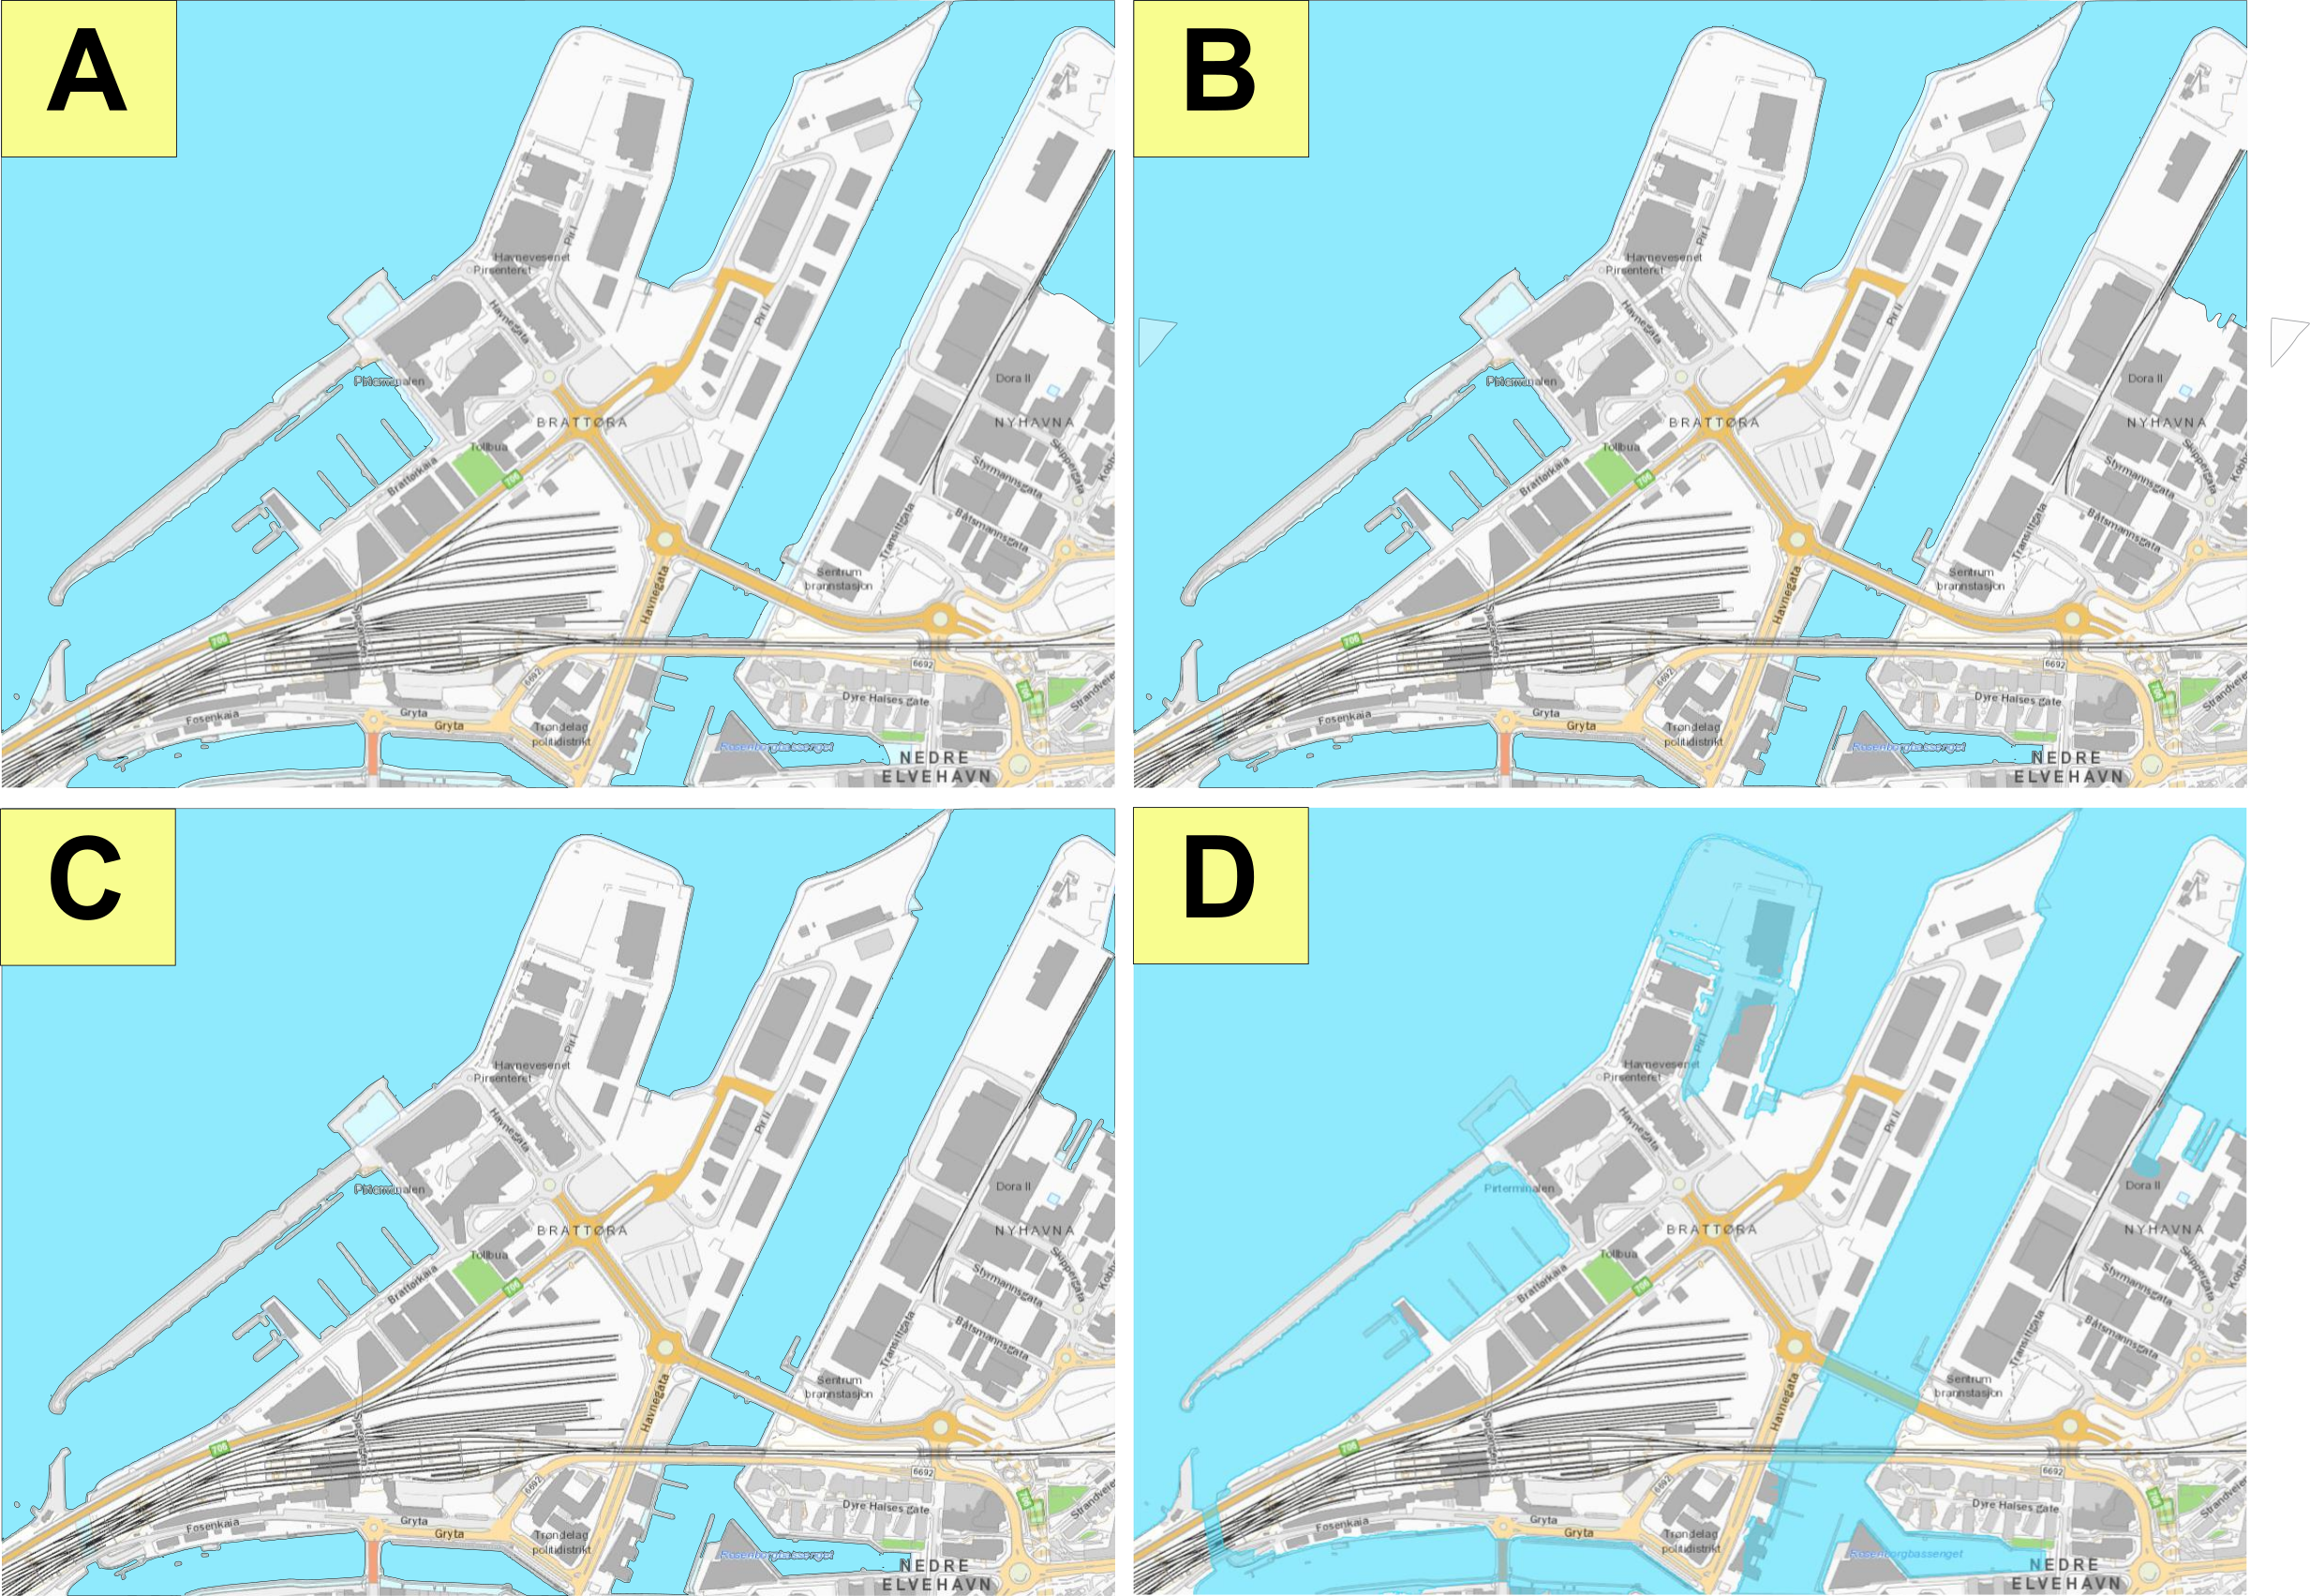
\includegraphics[width=8cm]{fig/brattora question on 2022 high tide quadrant.png}
    \caption{Which image displays Brattøra's High tide? -  This image contains four maps representing potential high tides in Brattøra. The map which matched models from \cite{kartverket_se_2021} is B. If subjects selected this response they were deemed aware of high tide in this place in the period 2022 to 2050. }
    \label{fig:Brattora_2022_hightide}
\end{figure}

\begin{figure}[h!]
    \centering
    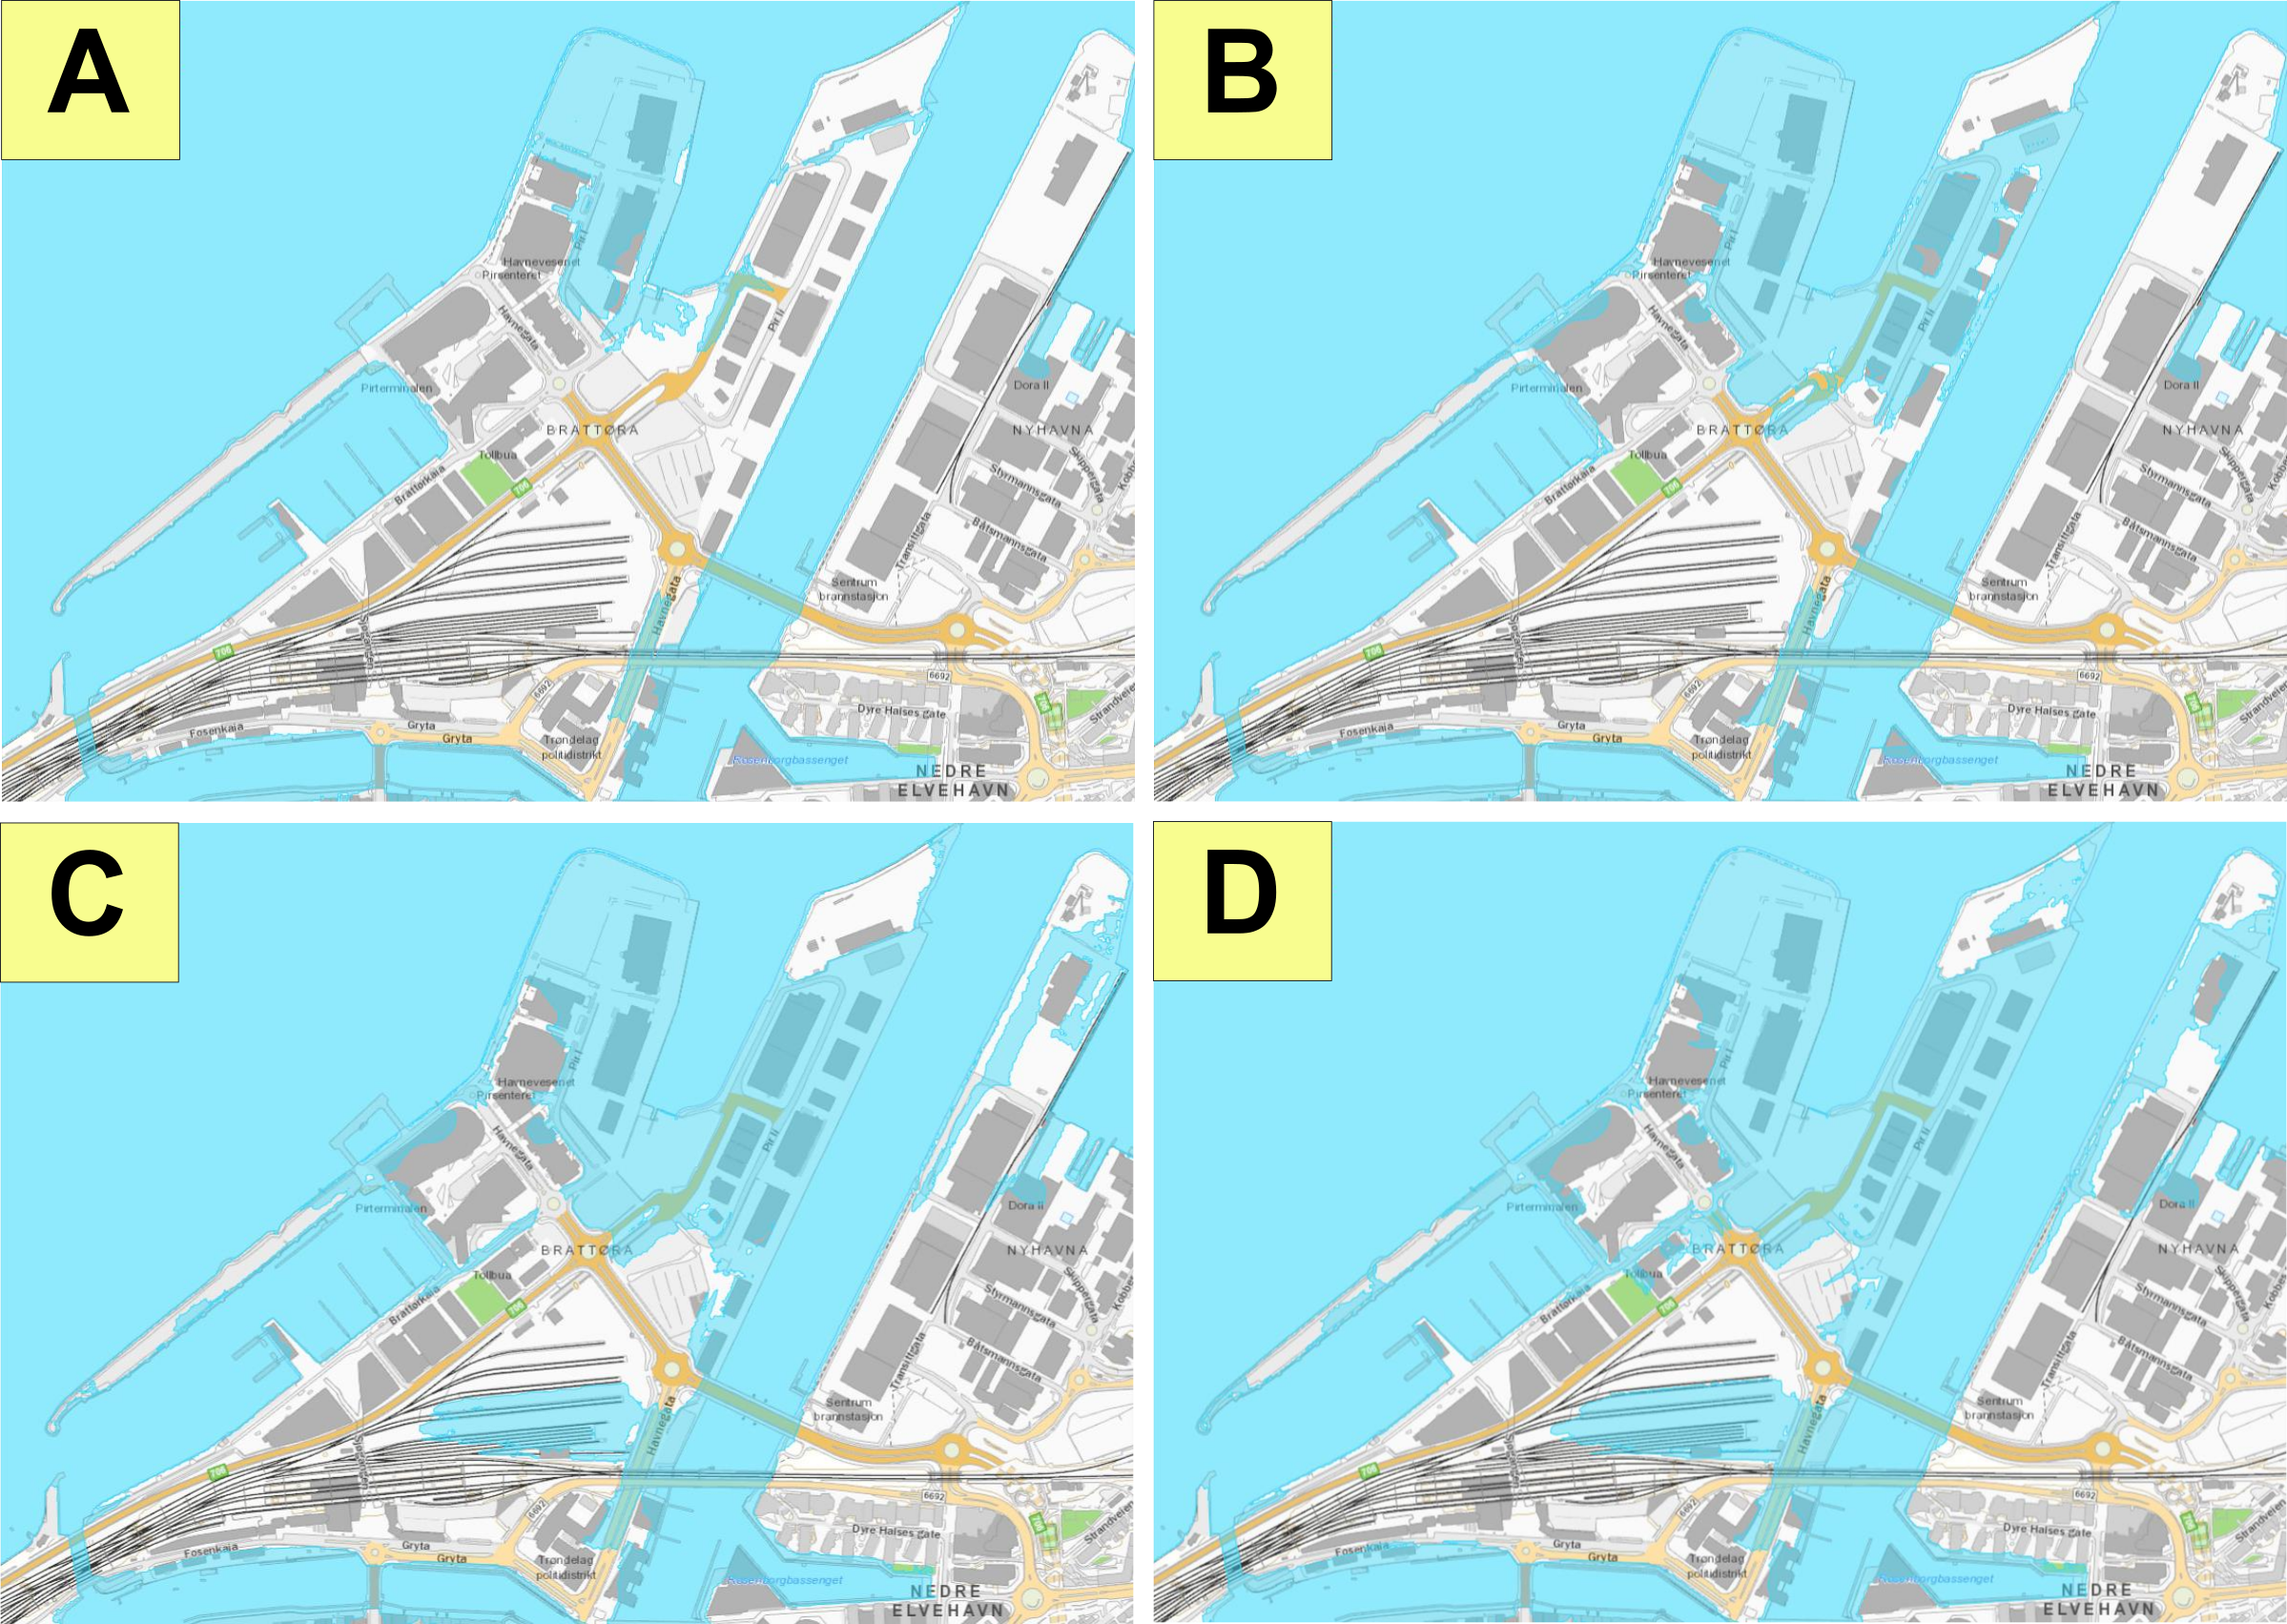
\includegraphics[width=8cm]{fig/brattora question on 2090 20 yr storm surge quadrant.png} 
    \caption{Which image displays Brattøra's 20 year storm surge in 2090? - This image contains four maps representing potential heights which could be caused by the 20 year storm surge. The map which matched the models from \cite{kartverket_se_2021} is B.If subjects chose this response they were deemed aware of the 20 year storm surge in the period 2050 to 2100. }
    \label{fig:brattora_2090_stormsurge}
\end{figure}

\begin{figure}[h!]
    \centering
    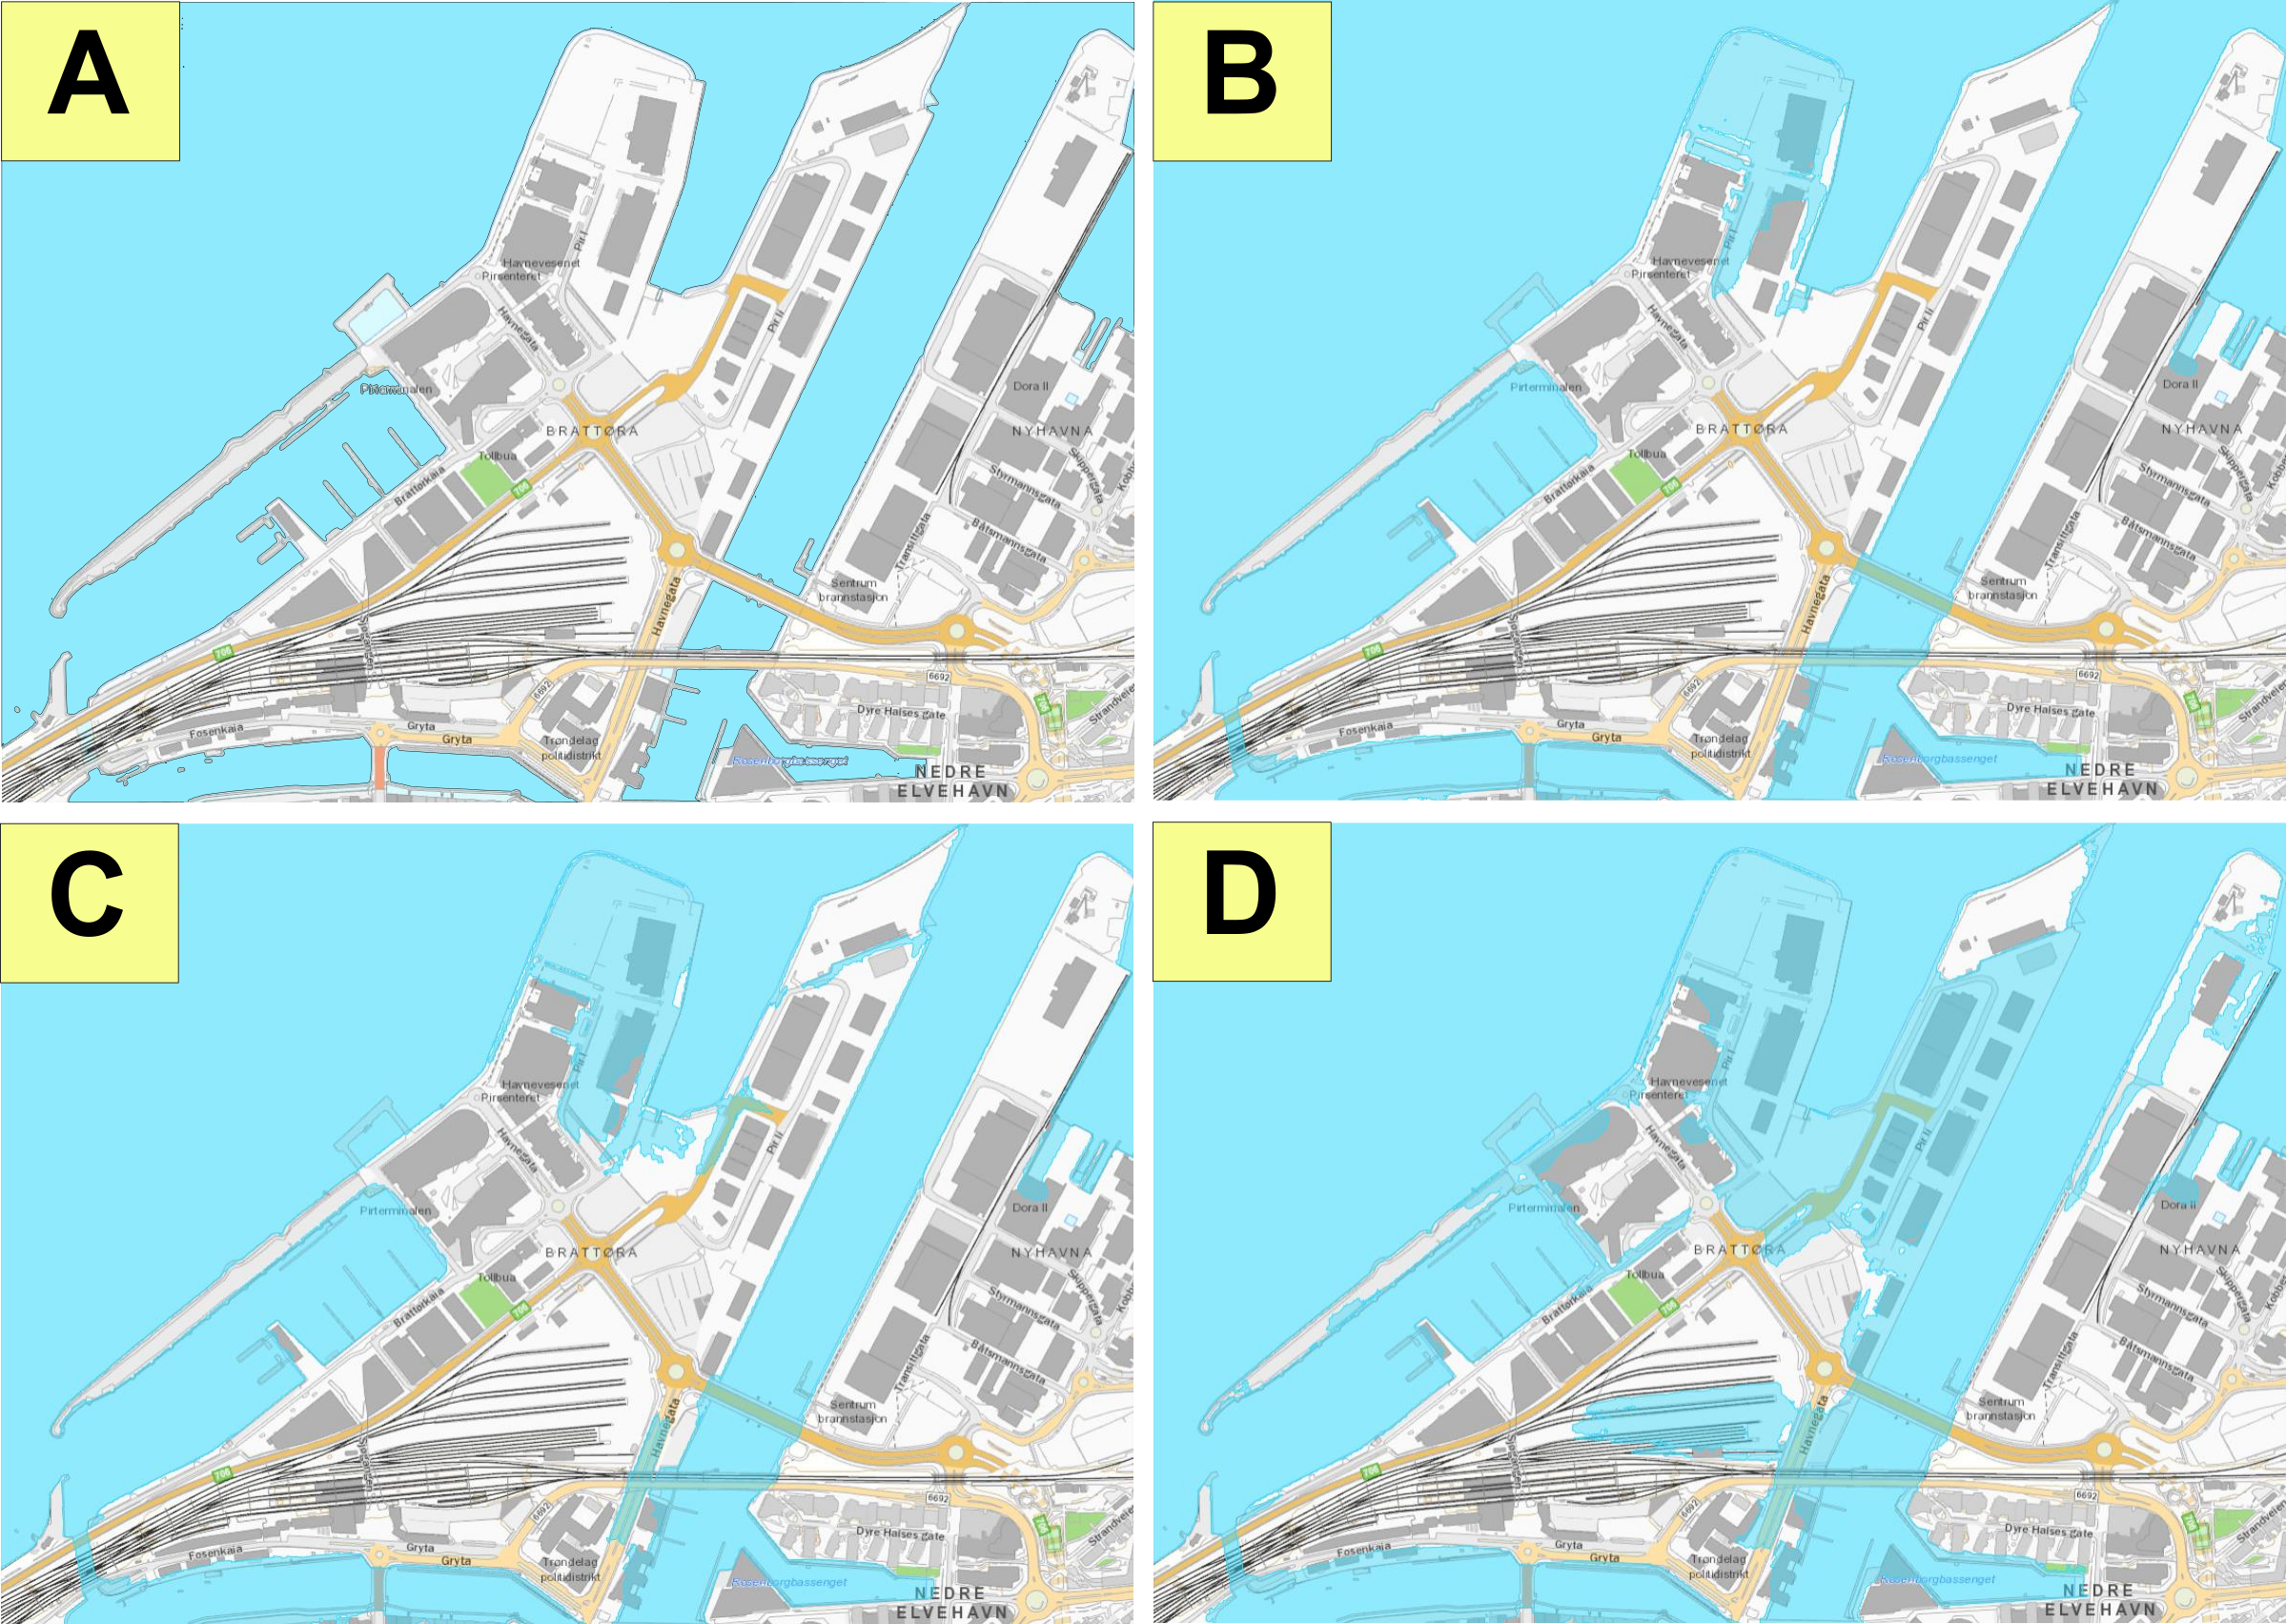
\includegraphics[width=8cm]{fig/brattora question on 2022 20 yr storm surge quadrant.png}
    \caption{Which image displays Brattøra's 20 year storm surge in 2022? - This image contains four maps representing potential heights which could be caused by the 20 year storm surge. The map which matched the models from \cite{kartverket_se_2021} is B.If subjects chose this response they were deemed aware of the 20 year storm surge in the period 2022 to 2050.}
    \label{fig:brattora_2022_stormsurge}
\end{figure}

The difficulty the participants had answering these questions is discussed in the results. After this a focus group was conducted including seven of the subjects from the pilot survey. The purpose of the focus group was to determine whether the subjects truly had high levels of awareness about sea level extremes and if so what prevented them from choosing the answer which corresponded with the models. The findings from the pilot survey and focus group were used to improve data collection methods. 

\section{Simulated Sea Level Extremes}
To determine Trondheim's social system a survey was carried out in the summer of 2022. A key purpose of this survey was to determine awareness of subjects. 
Five questions were asked to aid the determination of this awareness and of these questions three included four pictures of simulated sea level extremes for each of the research sites. These were created based of models form \cite{dsb_integrating-sea-level-rise-and-storm-surges--local-planningpdf_2017} and \cite{kartverket_se_2020}. Maps were created for various potential sea level extremes at the chosen research sites. The photos of the sites were taken to make understanding and editing as easy as possible. To do this the photos were taken on a sunny day, minimising people and boats, while attempting to capture recognisable landmarks of each of the sites. The exact geo-location and timing of the photos was noted to allow for determination of the water height. Table 3.1 below displays the water height of each of the original photos. 
\paragraph{}

\begin{table}[h!]
    \centering
    \begin{tabular}{|l|l|}
        \hline
     	Research Site & Photo water level (cm) \\ \hline
            Grillstad & 50 \\ \hline
            Skansen & -23 \\ \hline
            Nidelva & -159 \\ \hline
            Brattøra	& -42 \\ \hline
    \end{tabular}
    \caption{Water levels on day of photo taken for simulated sea level extremes this was determined from \cite{tides_high_2022}. Water levels included consideration of tide plus weather effects plus river levels}
    \label{tab:water_level_photo}
\end{table}
\paragraph{}

Using \cite{tides_high_2022} the water level for each of the original pictures was determined. For Skansen, Grillstad and Brattøra this meant combing the tides, plus weather effects. On most days to calculate Nidelva research site's water level would need to include the river level. However, time and day chosen was one with a particularly low river level which allowed for this value to be excluded as water level was dominated by the tide at the time of the photo being taken.   
\paragraph{}

These determined water levels was the base where each simulated water level could be added to. Table 3.2 and 3.3 below show the sea level extremes and the associated water level with NN2000 as a reference point.  To be able to relatively accurately add the simulated water levels to the images the first step is to make sure that each of the photos included a reference height. These key features (bins, fences, permanent benches, windows), were measured using a tape measure to allow for simulated realignment of the water levels to particular heights. Perspective was an important consideration in the original photos. Having the coastline at an angle allowed for a more realistic image, but did complicate the photo editing. 

\begin{table}[h]
    \centering
    \begin{tabular}{|l|l|l|l|l|l|}
    \hline
     Sea Level &   mean high  & mean high  & 20 year  & 200 year   & 1000 year  \\ \newline
     Extreme &  water neeps & water springs &  storm surge  & storm surge  &  storm surge  \\ \hline
       Height (cm) &  55 & 119 & 216 & 234 & 244 \\ \hline
    \end{tabular}
    \caption{2022 Sea Level Extremes Projections \cite{kartverket_se_2020}}
    \label{2022_sle_projections}
\end{table}

\begin{table}[h]
    \centering
    \begin{tabular}{|l|l|l|l|l|}
    \hline
       Sea Level &  mean high & 20 year   & 200 year &  1000 year   \\ \newline
       Extreme & water springs &  storm surge  &  storm surge  &  storm surge  \\ \hline
       Height (cm) & 172 & 269 & 286 & 297 \\ \hline
    \end{tabular}
    \caption{2090 Sea Level Extremes Projections \cite{kartverket_se_2020}}
    \label{2090_sle_projections}
\end{table}

Once the heights were calculated from the tables above they were drawn onto the original images using inkscape. This new image was then used as the base layers when simulating the extreme sea levels. To do this the original image was replicated twice using GIMP, GNU Image Manipulation Program, with a reduced opacity. The extra layer allowed for easier fixes during the next step. 
\paragraph{}
Next the top layer was then cut to leave only the water present in the image using the free select tool. If too much was cut the layer underneath could be used as a back up. After this the handle transformation tool was used on this layer to define points. This layer was then aligned for each of the draw upon water levels. Soft eraser tool was used to minimise oddities in the water created due to this movement. Dodge tool was used to darken below the water line to make the water line more distinct as calm bright days were chosen, meaning the edge of the water was difficult to pin point on small screens. Finally the clone tool was used to get ride of potential distractions, including seagulls and boats floating on the sea. Once satisfied the image was exported as a JPEG. 

\paragraph{}
The final values and water levels used were rounded to 10cm due to ease of participants understanding and to not give a false sense of accuracy in the images. The exported JPEGs were combined into grids and labelled for use in the survey. 



\section{Data Collection}

Data collection for this study comprised of two aspects.  The first involved literature reviews and collecting models of sea level rise and sea level extremes. The aim was to create a realistic visualisation of sea level extremes in Trondheim between 1950 and 2100 to utilise in discussion of awareness of sea level extremes. 
\paragraph{}

The second was an online survey conducted in the summer of 2022. The aim was to explore subjects experience, awareness and information access about sea level extremes and climate change. Subjects were recruited via social media, email and posters placed along Trondheim’s coastline focusing on locations where people wait. The survey was designed to take under five minutes to maximise responses. Stakeholders targeted were those with direct experience of Trondheim’s coast specifically the four places – Brattøra, Skansen, Nidelva and Grillstad. These locations were chosen after naturalistic observation along all populated areas of Trondheim’s coast. Trondheim was selected due to the potential to utilise personal network plus COVID-19 restrictions. These locations were chosen due to their high throughput of all demographics and perceived physical vulnerability. Nyhavana was not selected due to less population throughput at the time of data collection and as the major impact on sea level extremes is ongoing construction and related subsidence \cite{miljoenheten_og_byplankontoret_trondheim_kommune_9-notat-om-havnivastigning-og-stormflo---hensyn-i-arealplanlegging-nyhavnapdf_2020}




\section{Communication Design}

When utilising citizen science communication style is very important. This section details the various methods used to reach subjects and encourage them to participate. Accessibility, trust and legitimacy are important attributes with all citizen science, but even more so for when investigating subjects with a potential emotional impact \cite{tweddle_guide_2012}. A simulated image which shows a place a participant cares about as being impacted by a sea level extremes could result in a strong emotional impact. If this is not handled carefully this could turn the participant away from the survey and research on this in general.
\paragraph{}

To reach participants the researcher's personal network was used, as were A4 posters, social media and emails to relevant organisations and employers. The subjects were directed to a website containing details about the project and links to surveys on each research site.
\paragraph{}

The Web Accessibility Guidelines - \cite{henry_web_2022} and Story Map Accessible Design Principles - \cite{todd_liz_getting_nodate} were actively used during the creation of the website and online surveys. These guide good standards of visual communication and accessibility by varied pieces of technology including e-readers. The guideline used for text was the Principles for effective communication and public engagement on	climate change: A Handbook for IPCC authors - \cite{corner_a_principles_2018}. While not written for citizen science its advice for when discussing climate change and how to connect with people on these subjects was very useful. 
\paragraph{}

The design principles which were followed can be summarised as:
\begin{itemize}
    \item Make it as easy as possible to participate
    \item Utilize personal brand to enhance connection and trust
    \item Be succinct
\end{itemize}
\paragraph{}
These were created from the guidelines mentioned above plus the researcher's previous experience working in communications including training in visual communication. To enhance legitimacy the results of this project will be shared with interested subjects via the website which was created.
\paragraph{}
In the appendix you can find example emails, social media posts and the poster used to access subjects. The full survey in Norwegian and English is also attached to demonstrate how the communication guidelines were implemented. Attempts were made to keep both the English and Norwegian survey as close as possible to allow for easy comparison. However, direct translation is not always possible and the nuance and implication of word choices can have significant impact on the results. This was minimised by the researcher writing both surveys rather than relying on a translator and by getting it checked by several individuals with understanding of the topic.



\section{Data Analysis of Survey Results}
An exploratory data analysis was done then non parametric hypothesis testing was conducted utilising Rstudio. Histograms and Shapiro Tests were used to determine the distribution and dot plots were created to search for linear relationships. The results of the analysis were exported from R to excel for plotting .
\paragraph{}
The survey comprised of 26 questions addressing awareness, memory of sea level extremes, interest levels in sea level extremes, community membership, information access, length of residence, attitudes as well as space to highlight other place-based risks. 153 responses were collected. 30 percent of respondents had no memory of sea level extremes in Trondheim with 70 percent having memory of one or more event. A third (50/153) remembered the most recent sea level extreme in February 2020. The planned analysis was linear regression as awareness is considered continuous or linear mixed effect models as their may have been random effects. However, due to lack of linearity in original dotplots another method was also chosen.

\paragraph{}
The non parametric hypothesis testing method of Kruskal wallis rank sum tests were used due to the lack of obvious linearity, as as awareness is considered continuous and as the data was not normally distributed. Logistic regression was considered, but was decided against as how you would split awareness into a dummy variable would have been the most significant impact on the results. The survey data was taken directly from Nettskjema, codified using excel and then exported to R, which was used to analyse all quantitative data. The results of the analysis were then exported to excel for use of their graph templates.
\paragraph{}
Participant diversity is inherently biased when relying on goodwill, but a wide range of levels of interest in sea level extremes and community membership were surveyed including those who were not interested and who had limited knowledge of Trondheim’s coasts, as can be seen in the results. The original intention was to determine awareness as the ability to answer 5 questions. This would hopefully create a homoscedasticitic (i.e. the residuals have constant variance at every level of x) variable with independent and normally distributed residuals. However quick analysis of the data showed that this would not be the case.
\paragraph{}
  For example only 3 subjects answered correctly to the question "How much do you think the sea level has changed in the past 30 years?", creating a incredibly skewed distribution. For this reason this variable (slr-past) has been excluded from the main determination of awareness. This does not mean it is not considered in the answer to research question 2, but research question 3 requires a significant percentage being deemed aware. 
\paragraph{}
  A higher percentage answered correctly to the question "How much do you think the sea level will change in the next 30 years?". However this percentage was deemed insignificant and more due to luck as 2/7 answers were appropriate. For this reason this variable (slr-future) was also excluded for the determination of awareness as used to answer research question 3. However, it is used when answering research question 2. The other questions used to determine awareness utilised images with simulations of the sea level extreme, unlike these questions which solely used numeric values. This is another reason why only three questions were included in the determination of awareness in contrast with the original plan. The exclusion of these potential variables is discussed further in the discussion, particularly what it infers about the ability to visualise from a number. 
\paragraph{}
Awareness was calculated using the responses to the three questions "Which image shows the current 20-year storm surge?", "Which image shows the 20-year storm surge projected for 2090?" and "Which image displays the current high tide?". In the appendix the full survey in both Norwegian and English is attached, which shows how subjects received both numeric and visual representation of the sea level extremes when answering these questions. 


\section{Limitations}
The COVID-19 pandemic provided significant limitations to this research. This was the main factor in the decision to only use surveys and not complement with interviews for this investigation of Trondheim's resilience to sea level extremes. Furthermore, resilience is dynamic and the pandemic will have had impacts on Trondheim's resilience. The timeline of this as a masters project put limitations on the gathering of data, especially when considering the social system aspects of resilience. 
\paragraph{}
The data gathered limitations include the number of subjects and the impact of only surveying during the summer. The lack of marine workers within the subjects is a major limitation of this study, which should be corrected if repeated, but does not prevent an overview of local knowledge. Particularly important is the limitation of only having the results for one year, which creates a snapshot of resilience rather than considering how it is changing. Furthermore the exclusion of Nyhavvna from the research sites which is explained in the discussion framework does provide a limitation.  The final limitation is the analysis technique which was limited due to the skewed distribution of the survey results.

